\section{Motivation and System Model}
\label{chapter:system-model}

\begin{figure}[t]
  \centering
    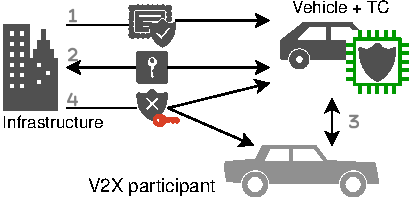
\includegraphics[width=.9\columnwidth]{figures/drawio/requirements.drawio.pdf}
  \caption{Lifecycle of a \acs{V2X} architecture. An infrastructure enrolls vehicles (1) and equips them with pseudonymous credentials (2) which they can use to take part in V2X communication (3). On-demand, the infrastructure revokes pseudonyms or certificates (4).}
  \label{fig:system-model}
\end{figure}

Section~\ref{related-work} highlights that, while active and passive revocation
schemes present some drawbacks, self-revocation of pseudonyms seems a promising
solution to remove misbehaving or malicious participants from the \ac{V2X}
network efficiently and in a timely manner. However, related work on the topic
ignores several challenges posed by realistic attackers and does not provide
strong guarantees or upper time bounds for revocation. None of the previous
papers effectively solved the problem of attackers actively dropping/delaying
revocation requests, and the \emph{heartbeat} idea was only informally
introduced but never
developed~\cite{whitefield2017privacy,desmoulins2019practical,larsen2021daa}. To
the best of our knowledge, there are no self-revocation schemes available that
work in practice, making these protocols unsuitable for real-world deployment in
\ac{V2X} systems. Earlier formal verification work~\cite{whitefield2017formal}
does not address this problem, and no related paper provides an upper-bound
analysis nor a comprehensive evaluation. Additionally, previous work hints at
the requirement of trusted timestamps in network messages, but none provides a
full design that integrates a trusted time source in \acp{TC}. In fact, under a
realistic attacker model, current confidential computing technologies, and
\acp{TEE} particularly, cannot rely on a trusted time
source~\cite{alder2023about}. Thus, previous works that implicitly assume
trusted synchronized time cannot currently be implemented securely.

In this work, we aim to
address these issues by providing a reliable, formally verified revocation
mechanism that can be employed in \ac{V2X} systems and beyond. We propose a
design that considers the challenges of having a reliable time source in
\acp{TC}, and we discuss optional extensions that may bring additional
advantages. We strive to minimize the computational and communication overheads
caused by revocation schemes, making our design efficient and suitable for any
kind of system and network. Below, we overview our system model, discuss
attacker capabilities, and introduce our objectives. Our design
is then detailed in \cref{chapter:design}.

\subsection{Vehicles and Trusted Components}
\label{section:trusted-component}

In \ac{V2X}, participants can be vehicles, pedestrians, traffic lights, and so
forth. For readability, in this paper we only discuss vehicles, but our system
model can be generalized to \emph{any} participant in the network. We consider
vehicles as integrated systems composed of a number of \acp{ECU} connected by a
local in-vehicle network such as a CAN bus. These \acp{ECU} may also be
connected to a wide variety of sensors and actuators, used to retrieve
information from the vehicle itself or its surroundings (e.g., speed, position),
or to perform actions (e.g., accelerate, brake). Typically, all such components
are managed by a central unit called \ac{OBU}, which is also responsible for
processing network messages sent to and from the
vehicle~\cite{liu2017invehicle}.

Additionally, we assume that vehicles contain a secure processing element called
the \acf{TC}, responsible for credential management and cryptographic
operations, analogously to \ac{DAA} protocols (cf.~\cref{background:v2x}). In
our system model, the \ac{TC} is a passive device that exposes an interface to
the \ac{OBU} for tasks such as enrollment/attestation, pseudonym generation, and
message signing/verification. Therefore, all sensitive operations are performed
on the \ac{TC} itself, and the \ac{OBU} cannot directly access cryptographic
keys or other sensitive material. Examples of \acp{TC} are the \ac{TPM}, ARM
TrustZone, or \acp{TEE} such as Intel \ac{SGX} and ARM \ac{CCA}. Nowadays,
trusted components are ubiquitous in modern hardware~\cite{schneider2022sok},
and with recent developments in the automotive domain, starting with Infineon's
automotive-certified Optiga TPM~\cite{optigaTPM} (released in 2018) and
automotive security processors such as the NXP NCJ38A~\cite{NXPsecureElement}
(available since 2020), \ac{TEE} solutions are available and working groups
within the Trusted Computing Group and Global Platform are active in designing
automotive security services based on
\acp{TEE}~\cite{TCG,GlobalPlatformAutomotive}.\gianluca{can we find better references?}

In our attacker model (cf.~\cref{section:attacker-model}), we consider all
components of the vehicle potentially malicious or compromised, except the \ac{TC}.
Therefore, at high level, we can define a vehicle as the sum of two main
components: the \emph{untrusted host} and the \ac{TC}. Just like sensors, timing
components used for precise timestamping are also part of the untrusted host,
such that the \ac{TC} cannot rely on a trusted notion of time by
itself~\cite{alder2023about,anwar2019applications}. Therefore, our design does
not assume a trusted time source in vehicles to guarantee a timely revocation,
but relies on trusted timestamps (or "epochs") distributed by the \ac{ITS}
infrastructure to \acp{TC} (cf.~\cref{chapter:design}).

\subsection{The Vehicle Lifecycle in a \ac{V2X} Network}
\label{section:system-model}

The lifecycle of a vehicle in a \ac{V2X} network is depicted in
\cref{fig:system-model} and, in short, is composed of four main phases:
%
\begin{inparaenum}
    \item \emph{enrollment},
    \item \emph{pseudonym generation},
    \item \emph{operation}, and
    \item \emph{revocation}.
\end{inparaenum}
%
Although our paper mainly focuses on the last phase, every revocation scheme, to
be effective, has some dependencies on the other phases. For example, vehicles
that do not properly check the validity of signatures might erroneously accept
messages signed with invalid or revoked pseudonym certificates, making the
revocation process useless. Thus, in this section we first compile a set of
functional requirements that a \ac{V2X} protocol should implement in order to
use our revocation scheme effectively. These requirements are based on the
architectures proposed in state-of-the-art \ac{V2X} credential management
systems, and are discussed at \emph{high level}: Our goal is to make our
revocation scheme protocol-agnostic in order to be compatible with most existing
protocols such as \ac{DAA} or technical standards such as ETSI and SCMS
(cf.~\cref{section:discussion-compatibility}).

\noindent\textbf{\emph{Enrollment.}} Each vehicle is equipped with a \ac{TC}
which exclusively stores credentials and performs cryptographic operations with
them (cf.~\cref{section:trusted-component}). In the initial phase, a vehicle
enrolls to the \ac{V2X} network by authenticating to the infrastructure, e.g.,
by presenting a valid certificate~\cite{etsi2022102941}. With trusted components
such as \acp{TEE}, \emph{remote attestation} also becomes an essential step to
make sure that the \ac{TEE} is configured correctly and is up to date, and the
\ac{TC} is running genuine software~\cite{schneider2022sok}. Successful
enrollment should result in the issuance of a \emph{long-term credential}, used
by the vehicle as a token to authenticate subsequent requests to the
infrastructure and to obtain pseudonym certificates (cf.~\cref{background:v2x}).
%
\begin{req}
    \label{req:enrollment}
 Vehicles correctly enrolled to the network are issued a long-term credential,
 stored in the \ac{TC}.
%  \eddy{Better layout is needed to indicate the requirement 1 is a summary of the previous paragraph}
%  Fritz: I see what you mean but it should become obvious from the next paragraphs that all have the same style
\end{req}
%

\noindent\textbf{\emph{Pseudonym generation.}} In this phase, a vehicle uses the
long-term credential obtained during enrollment to get a new pseudonym
certificate. This process can be done either \emph{online}, where the pseudonym
is issued by the infrastructure upon successful
authorization~\cite{etsi2022102941,brecht2018scms}, or \emph{offline}, where the
vehicle's \ac{TC} performs a key derivation from the long-term
credential~\cite{whitefield2017privacy,desmoulins2019practical}. Either way,
only non-revoked vehicles should be able to obtain new pseudonyms.
%We also require that pseudonyms have a unique and public identifier (e.g., a
%hash of the public key).
%
\begin{req}
    \label{req:pseudonym}
    Pseudonym certificates are obtained using (valid) long-term credentials
    through online or offline protocols. 
    %Each pseudonym should have a unique public identifier.
\end{req}
%
\noindent\textbf{\emph{Operation.}} Pseudonyms are then used to authenticate
messages that vehicles exchange with network peers. For readability and without
loss of generality, this paper focuses on the communication between vehicles
(\ac{V2V}), but peers could also be pedestrians (V2P), smart city infrastructure
(V2I), and so forth (cf.~\cref{chapter:background}). \ac{V2V} messages may
include information about the vehicles themselves (e.g., speed, location,
direction) and the surrounding environment (e.g., traffic, accidents). These
messages need to be integrity-protected and authenticated to prevent message
spoofing or tampering, and time-stamped to provide freshness; Both actions are
performed by the \ac{TC}, using pseudonym credentials for the former and its
internal time \funcnow{} for the latter (we elaborate more on \funcnow{} in
\cref{chapter:design}).

\begin{req}
    \label{req:v2v-send}
    \ac{V2V} messages are signed by the \ac{TC} using its own valid pseudonyms
   and timestamped according to an internal \ac{TC} variable \funcnow{},
   representing the \ac{TC}'s current time.
\end{req}
We then require that vehicles correctly check the authenticity of \ac{V2V}
messages to ensure that they have been signed using a valid pseudonym
certificate. Furthermore, we demand that messages older than a predefined age
are discarded, to prevent processing outdated information.
%
\begin{req}
    \label{req:v2v-receive}
    Vehicles should check the signature of received \ac{V2V} messages to ensure
    that they have been generated using a valid pseudonym. A message with
    timestamp \paramtvv{} should only be accepted by a receiving \ac{TC} if not
    older than a predefined window \paramtt{} w.r.t.~its internal time
    \funcnow{}:
    %
    \begin{equation}
        \label{eq:valid-v2v-generic}
        \paramtvv \geq \funcnow - \paramtt
    \end{equation}
    %
\end{req}
%
%We will come back to \cref{eq:valid-v2v-generic} in \cref{chapter:design}.

\noindent\textbf{\emph{Revocation.}} We expect the infrastructure to operate
mechanisms for misbehavior detection and reporting, where pseudonyms can be
flagged, e.g., for spreading messages that contain false
information~\cite{brecht2018scms,etsi2020tr103460}. Based on such reports, the
\ac{RA} can decide to revoke the corresponding vehicle's credentials using the
reported pseudonym. This is the concept of \emph{message-based revocation}
introduced in \cref{chapter:background}.
%
\begin{req}
    \label{req:revocation}
    The \ac{RA} makes decisions on revocation by employing misbehavior detection
    mechanisms in the network, to identify and report misbehaving pseudonyms.
\end{req}
Moreover, we require that \emph{only} non-revoked vehicles can enroll to the
network, otherwise it would be trivial for attackers to bypass revocation by
simply re-enrolling to the network. This can be achieved by keeping an internal
blacklist of long-term credentials~\cite{etsi2022102941,brecht2018scms}. Revoked
vehicles may be reinstated at the discretion of the \ac{ITS} infrastructure,
e.g., after a factory reset.
%
\begin{req}
  \label{req:revoked}
    Only vehicles whose credentials have not been revoked can (re-)enroll to the
    \ac{V2X} network.
\end{req}
%
We observe that a vehicle in a \ac{V2X} network is operational iff two
conditions are fulfilled:
%
\begin{inparaenum}
    \item the vehicle has \emph{at least} one valid pseudonym, and
    \item the \ac{TC}'s internal time \funcnow{} is loosely synchronized with
    the others, i.e., within window \paramtt.
\end{inparaenum}
%
If either of these two conditions is not met, a vehicle cannot generate valid
and fresh \ac{V2V} messages, according to \cref{req:v2v-send,req:v2v-receive}.
Hence, we define \emph{effective revocation} as follows:
%
\begin{defn}[\emph{effective revocation}]
A vehicle is considered effectively revoked when either all its pseudonyms are
made unusable (or expire), \emph{or} when its \ac{TC} gets permanently
de-synchronized, i.e., when \funcnow{} cannot be updated anymore.
\end{defn}


% In \cref{chapter:design} we describe how our design achieves this goal.

\subsection{Attacker Model}
\label{section:attacker-model}

We consider a powerful attacker that has control over a vehicle with valid
credentials and wants to disrupt the \ac{V2X} network by spreading malicious
\ac{V2V} messages, avoiding revocation of their pseudonyms as long as possible.
Examples of attack vectors include faulty sensors, software bugs in \acp{ECU}, root
access to the attacker's own car, etc.

We assume a Dolev-Yao style attacker that controls the network stack and can
tamper with, rearrange, resend, and stall network messages but not break
established cryptography~\cite{dolev1983security}. The attacker is assumed to
have full control over all hardware and software on vehicles except for
functionality implemented by their \ac{TC}, which is protected and fully
trusted. Entities in the \ac{ITS} infrastructure (e.g., the \ac{RA}) are also
trusted.

Besides the aforementioned cryptographic limitations, our attacker is not able
to perform physical attacks on the \ac{TC}.
%As the current time is an essential element when discussing pseudonym
%revocation, the attacker is also not assumed to be capable of over- or
%underclocking the time source of the \ac{TC}. While this is a form of physical
%attack that has to be dealt with via physical hardening of the hardware, we
%acknowledge the danger this attack vector imposes on potential protocols. Thus,
%our second protocol\christoph{only one} does not fall under this restriction
%and is independent of hardware time sources. 
We stress that voltage tampering attacks against the hardware can still be a
real threat and cannot be tackled by network protocols, but need to be addressed
on lower levels of the stack~\cite{chen2021voltpillager,
murdock2020plundervolt}. Side channel attacks against the \ac{TC} are also out
of scope and will have to be mitigated through the usual means of hardware and
software defenses~\cite{lou2021survey, canella2019systematic}.

\subsection{Objectives}
\label{section:system-objectives}

Based on our system and adversary model, and the open issues of existing schemes
(cf.~\cref{related-work}), we define objectives for a practical and secure
real-world revocation mechanism:

\begin{enumerate}
  \item[{\crtcrossreflabel{\textbf{O1}}[obj:revocation]}] \textbf{Guarantee of
  revocation:} Revocation should always succeed within a deterministic upper
  bound, even in case of delayed or dropped revocation requests. In particular,
  the \textit{effective revocation time} is a time period starting with the
  revocation decision made by the \ac{RA} and ending when the vehicle is
  effectively revoked.
  \item[{\crtcrossreflabel{\textbf{O2}}[obj:trusted-time]}] \textbf{No
  assumptions on trusted time:} Synchronizing trusted time across multiple
  vehicles with a strong attacker is challenging and no assumptions should be
  made on having access to a local trusted time source.
  \item[{\crtcrossreflabel{\textbf{O3}}[obj:scalability]}] \textbf{Scalability:}
    Any revocation mechanism suitable for \ac{V2X} scenarios must be scalable in
    terms of vehicles and share of attackers in the network. This covers both
    computational as well as network overhead.
  \item[{\crtcrossreflabel{\textbf{O4}}[obj:adaptability]}]
  \textbf{Adaptability:} The revocation mechanism needs to be configurable for
  different network characteristics and security requirements. It must be able
  to tolerate varying degrees of network latency.
  % I removed the 'accommodate for long network latencies.'
\end{enumerate}

%%TODO GS: I commented the paragraph below because from 4.1 it should now be
%%        clear what we mean by effective revocation
%We note that \ref{obj:revocation} does not necessarily involve deletion of
%credentials, as \acp{TC} could have impaired communication capabilities.
%Instead, we require that \emph{all} network participants eventually discard any
%messages signed with revoked pseudonyms, thus making pseudonym revocation a
%property of the network instead of the individual \acp{TC}.
%\christoph{it takes quite some time to finally get to the meat and main idea, maybe explain it %earlier?}
